\section{Introduction}

The proposed problem consists of a wall composed by two materials of different thermal conductivities, with a prescribed heat flow $q'' =$ \SI{6000}{W/m^2} on the left border, and a convective heat flow on the right border, with $h =$ \SI{100}{W/m^2.K} and $T_\infty =$ \SI{40}{\celsius}.
For this case, steady state is assumed.

\begin{figure}[h]
    \centering
    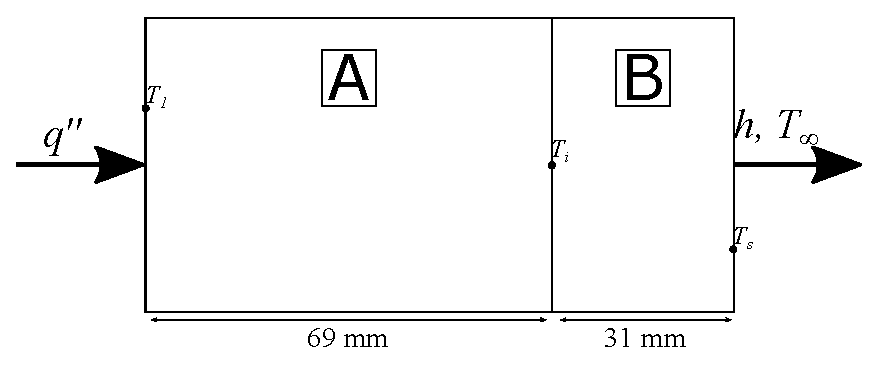
\includegraphics[scale=1]{problema.eps}
    \caption{Schematic representation of the problem.}
    \label{fig:problema}
\end{figure}

By making an energy balance at the borders and at the contact interface, the exact values of the analytical solution of the problem are easily found:

\begin{equation*}
    q'' = \frac{k_A \left(T_1 - T_i \right)}{L_A} = \frac{k_B \left(T_i - T_s \right)}{L_B} = h \left(T_s - T_\infty \right)
\end{equation*}

\begin{equation*}
    \SI{6000}{W/m^2} =
    \frac{10 \left(T_1 - T_i \right)}{0,069} =
    \frac{1  \left(T_i - T_s \right)}{0,031} =
    100 \left(T_s - 40 \right)
\end{equation*}

\begin{align*}
    T_1 &= \SI{327.4}{\celsius} \\
    T_i &= \SI{286}{\celsius} \\
    T_s &= \SI{100}{\celsius}
\end{align*}

For the numerical solution of the temperature profile, it is necessary to discretize the differential equation obtained by an energy balance (Equation \ref{eq:eqdif}), also applying the two boundary conditions (Equations \ref{eq:cc1} and \ref{eq:cc2}).

\begin{align} 
    \diff{}{x} \left( k \diff{T}{x} \right) &= 0 \label{eq:eqdif} \\
    -k \left. \diff{T}{x} \right|_{x = 0} &= q'' \label{eq:cc1} \\
    -k \left. \diff{T}{x}\right|_{x = L} &= h \left(T_s - T_\infty \right) \label{eq:cc2}
\end{align}

Discretizing the domain in $N_A$ control volumes for the $A$ part and $N_B$ control volumes for the $B$ part, placing the mesh points at the domain boundaries, a mesh is obtained as in the figure \ref{fig:mesh}.
The points in the $A$ part are separated by a distance $\delta x_A$ and the points in the $B$ part are separated by a distance $\delta x_B$, calculated according to the equations below:

\begin{equation*}
    \delta x_A = \frac{L_A}{N_A - 0,5} \qquad\qquad \delta x_B = \frac{L_B}{N_B - 0,5}
\end{equation*}

\begin{figure}[h]
    \centering
    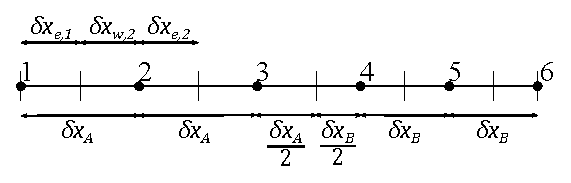
\includegraphics[scale=1.2]{mesh.eps}
    \caption{Schematic representation of the mesh.}
    \label{fig:mesh}
\end{figure}

For points within the mesh, the discretization by the finite volume method for an arbitrary point $P$, in this case called $i$ is given by the equations below, with point $i + 1$ equivalent to point $E$ (East), and the $i-1$ point equivalent to the $W$ (West) point:

\begin{align*}
    a_p T_P &= a_e T_E + a_w T_W \\
    a_i T_i &= a_{i+1} T_{i+1} + a_{i-1} T_{i-1} \\
    a_e &= a_{i+1} = \frac{k_e A}{\delta x} = \frac{k_e A}{\delta x_{e,i} + \delta x_{w,i+1}} \\
    a_w &= a_{i-1} = \frac{k_w A}{\delta x} = \frac{k_w A}{\delta x_{w,i} + \delta x_{e,i-1}}\\
    a_p &= a_i = a_{i+1} + a_{i-1}
\end{align*}

Where $k_e$ and $k_w$ for neighboring volumes with different thermal conductivities are calculated by linear variation or by the formulation of thermal resistances:

\begin{align*}
    k_{e, \text{linear}} &= f_e k_P + (1 - f_e) k_E = f_e k_i + (1 - f_e) k_{i+1} \\
    k_{e, \text{resistances}} &= \left(\frac{1 - f_e}{k_P} + \frac{f_e}{k_E} \right)^{-1} = \left(\frac{1 - f_e}{k_i} + \frac{f_e}{k_{i+1}} \right)^{-1} \\
    f_e &= \frac{\delta x_{w,E}}{\delta x} = \frac{\delta x_{w,i+1}}{\delta x_{w,i+1} + \delta x_{e,i}} \\
    k_{w, \text{linear}} &= f_w k_P + (1 - f_w) k_W = f_w k_i + (1 - f_w) k_{i-1} \\
    k_{w, \text{resistances}} &= \left(\frac{1 - f_w}{k_P} + \frac{f_w}{k_W} \right)^{-1} = \left(\frac{1 - f_w}{k_i} + \frac{f_w}{k_{i-1}} \right)^{-1} \\
    f_w &= \frac{\delta x_{e,W}}{\delta x} = \frac{\delta x_{e,i-1}}{\delta x_{e,i-1} + \delta x_{w,i}}
\end{align*}

For the first boundary condition (prescribed heat flux), applying finite volume discretization and integrating the differential equation, an algebraic equation is obtained as follows:

\begin{align*}
    a_p T_P &= a_e T_E + b \\
    a_1 T_1 &= a_2 T_2 + b \\
    a_p &= a_e = \frac{k_e A}{\delta x} = \frac{k_e A}{\delta x_{e,1} + \delta x_{w,2}} \\
    b &= q'' A = 6000
\end{align*}

For the second boundary condition, the discretized equation is obtained in the same way, arriving at the equations shown below, where $N$ is the last point of the mesh ($N = N_A + N_B$).

\begin{align*}
    a_p T_P &= a_w T_W + b \\
    a_N T_N &= a_{N-1} T_{N_1} + b \\
    a_w &= \frac{k_w A}{\delta x} = \frac{k_w A}{\delta x_{e,N-1} + \delta x_{w,N}} \\
    a_p &= a_w + h A \\
    b &= h A T_\infty = 4000
\end{align*}

With all the equations discretized, a $N \times N$ matrix is constructed with the linear coefficients $a_p$, $a_e$ and $a_w$ for each point of the mesh in each line of the matrix, thus generating a tri-diagonal matrix.
From the two boundary conditions, the column matrix of independent terms of the linear system is constructed, given by the prescribed heat flow and the convective coefficient with its respective external fluid temperature.
Then, the system of equations can be solved using the internal \emph{MATLAB} algorithms, finding the temperatures at each point in the mesh.
As an example, for the mesh represented in Figure \ref{fig:mesh}, the system of equations is:

\begin{equation*}
    \begin{bmatrix}
             362,3188 & -362,3188 &         0 &         0 &         0 &         0  \\
            -362,3188 &  724,6377 & -362,3188 &         0 &         0 &         0  \\
                    0 & -362,3188 &  494,2450 & -131,9261 &         0 &         0  \\
                    0 &         0 & -131,9261 &  212,5713 &  -80,6452 &         0  \\
                    0 &         0 &         0 &  -80,6452 &  161,2903 &  -80,6452  \\
                    0 &         0 &         0 &         0 &  -80,6452 &  180,6452
    \end{bmatrix}
    \cdot
    \begin{bmatrix}
        T_1 \\
        T_2 \\
        T_3 \\
        T_4 \\
        T_5 \\
        T_6
    \end{bmatrix}
    =
    \begin{bmatrix}
        6000 \\
        0 \\
        0 \\
        0 \\
        0 \\
        4000
    \end{bmatrix}
\end{equation*}